\chapter{Process}

%********************************** %First Section  **************************************
\section{Diagnostic} 

The idea of exploring the topic of testing in a Dynamics 365 for Finance and Operation environment was firstly introduced in order to compensate the lack of definition of a proper methodology to follow during the development of a project in order maintain high standards of quality and reliability. 
At the beginning of this work we explained how the purpose of the Diagnostic phase was the creation of a project plan that would allow us to form an initial determination of the project requirements together with their scope and the amount of time to dedicate to each activity. This allowed us to better understand how many resources needed to be allocated for the completion of the project and gave us a tool to monitor to which degree we were able to respect the predefined timeline. In this section we will not provide further information regarding the structure of the plan (section 1.4.2) and the defined requirements (Chapter 2).

A secondary activity was setting up the environment that would later be used to access the development tools. The company account was created and given access to the Trade+ project on Azure DevOps. A dev virtual machine was also set up and the Visual Studio Environment was connected to the project using Visual Studio Team Explorer.

Relevant links were provided in order to access the Dynamics Learning Portal, Lifecycle Services, Microsoft Developers Network, the company Intranet and the Trade+ project portal.

%********************************** %Second Section  **************************************
\section{Analysis} 

The identification of the activities that had to be covered by test cases was mainly based on finding a balance between the skills acquired since the beginning of the work and the usefulness of the tested tasks. As mentioned before (Section 1.4.2) we settled on five processes that had to be analyzed in order to have a satisfactory output (both in terms of coverage and documentation) at the end of the project. Said processes, together with steps that compose them, read as follows:

\begin{itemize}
    \item \textbf{Purchase Order}. Creation of new license plates to identify the purchased goods, creation of a new PO (with vendor and arrival site and warehouse), specification of items number and quantity, order confirmation, specification of order lines, baydoor registration, creation of product receipt (with id), posting of product receipt, invoice creation, invoice posting.
    \item \textbf{Production Order}. Creation of PO (with item number, delivery date and quantity), validation of PO, update of BOM (bill of materials) and production route, estimation and cost management, scheduling/release/start of production, reporting of production as finished (with publishing of journal entry). 
    \item \textbf{Transfer Order}. Creation of TO (with origin and target warehouse), specification of items number and quantity, inventory reservation, items picking from origin warehouse, items shipping to target warehouse, receival confirmation.
    \item \textbf{Sales Order}. Moving items from receival area to storage (transfer journal), creation of a new SO (with customer account and origin site and warehouse), specification of items number and quantity, inventory reservation, release to warehouse (creation of work item), validation and completion of work, creation of shipping load, shipment.  
    \item \textbf{Return Order}. Creation of RO (with customer account, return site and warehouse and return reason code), specification of items number and quantity, specification of order lines, baydoor registration.
\end{itemize}

After this initial definition we also decided that it would be appropriate (as a secondary step) not only to test the processes in isolation (feature testing) but also as single coherent workflow (integration testing) in which multiple tasks are interconnected with one another [Figure \ref{fig:processesWorkflow}]

\begin{figure}[ht]
	\centering
	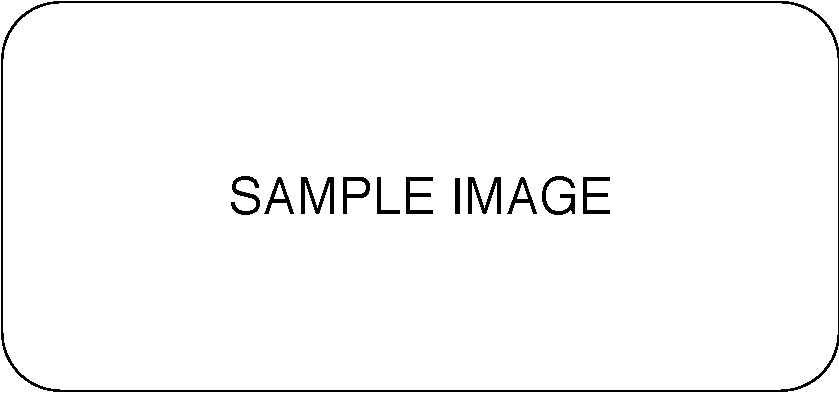
\includegraphics[scale=0.7]{Images/SampleImage.pdf}
	\caption{Processes workflow}
	\label{fig:processesWorkflow}
\end{figure}

The Analysis phase was also characterized by a series of training activities (mentioned in section 1.3) that were organized in order to give a satisfactory introduction to the world of ERP application and naturally had a particular focus on the Dynamics suite. The "Introductory lectures for new hires" are carried out with regularity by the company and aim to form the new team members to the internal practices, policies and tools. During the first weeks the following lectures were organized: Introduction to Dynamics, look and feel of Dynamics 365, Sales and logistics, production, development process overview and introduction to Trade+. On the Dynamics Learning Portal we followed the set of lectures called "Development, Extensions and Deployment for Microsoft Dynamics 365 for Finance and Operations" (Exam MB6-894) that covered: The understanding of Dynamics 365 for Finance and Operations architecture (application stack, cloud components, server architecture, layers) and development environment (Visual Studio and Lifecycle Services), development of new elements (creation and management of data types, tables and labels), the X++ programming language, user interface and security and component extension. Additional (independent) lectures were also followed on the topics of: System architecture and technologies (80765BE), cloud deployment (81144AE), advanced security (80929BE) and DevOps testing/practices/principles (Steven Borg, Sam Guckenheimer).

%********************************** %Third Section  **************************************
\section{Design} 

Dynamics 365 for Finance and Operations provides a easy-to-use tool (the Task Recorder) to record business processes and download them as .xml or .axtr files. The tool is integrated in the browser client and when activated records every user interaction with the system creating a step-by-step list of the performed actions. Each step appears to the user as a human readable, high level description of the action that has been performed (e.g. In the Warehouse field, type '6') and, once the recording file is downloaded, corresponds to a portion of the XML code that provides the system with information on the actions that have to be performed on the application. The recording process can be interrupted and resumed at any point and every created step can be commented (to provide further information to the users that will look at the interested recording), modified or deleted. A downloaded recording can be saved in the Lifecycle Service portal as a guide (.axtr), played back and edited by another user in his Dynamics environment (.axtr or .xml) and converted into a test case (.xml). The playback functionality is particularly useful to guide developers when a bug (that triggers after a series of specific actions) needs to be fixed. Because of this reason the recordings are usually created by consultants and attached to Azure Boards work items. Said items (as mentioned in section 4.2) are assigned to developers that can later download and use the attached recording file to emulate the interested behavior on their personal environment in order to better understand the problem without having to rely only on a written description of it.

After an initial period, necessary in order to get accustomed with the tool, we started to plan the recording activities. A major focus during this phase was the reduction of the steps needed to cover the interested business processes. These "simplification" tasks were of particular importance to reduce the amount of code that a given recording would generate when converted into a coded test case. A shorter test case is easier to maintain, expand and modify. Furthermore superfluous steps would have increased the likelihood of unexpected errors and behaviors. Other than reducing the total number of steps we also made sure that each recording could be played back on any machine running the same version of Dynamics 365 for Finance and Operations, independently from the underlying status of the database at the start of the execution. This meant encompassing all the activities related with the creation of the needed data at the beginning (or during) the interested business process (e.g. If a license plate needs to be used, create it before using it). Some information (like the predefined item selected in a drop-down menu) is also saved locally by Dynamics 365 for Finance and Operations and depends on how the user has previously interacted with the system. This peculiarity had to be taken into consideration during the recording activities in order to create file that could be played back (and later executed) on any machine (e.g. make sure that each item in a form is explicitly defined during the recording, etc.). 

Regarding the business processes covered in our work we decided to create a single recording for each activity, ending the Design phase with five .xml files that could later be utilized to create the foundation for our test cases. Another option that we considered was to cover all the core activities that needed to be tested in a single session. This approach would have resulted in the creation of a single recording file (and consequently in a single test case) thus simplifying the communication between the various business processes. Despite this fact, having a single test case would have greatly reduced the granularity that we would have during the execution of multiple test cases. Because of this reason this approach was later rejected.


%********************************** %Fourth Section  **************************************
\section{Development} 

This section covers all the Development tasks that were carried out during the course of our work. We decided to organize it into three subsections corresponding to the different macro-activities of this phase (mentioned in section 1.4.2). The first subsection describes the creation of the project that hosted our code and the translation of the task recordings into coded test cases. The secon one provides information regarding how said test have been expanded in order to fulfill the testing requirements of the application. Finally, the last subsection describes the process of integrating the test cases with the nightly builds.

\subsection{Creation}

As mentioned before (section 4.1) the handling of Dynamics 365 for Finance and Operations elements is done via a project that needs to be tied to a single model. Because of this reason, at the beginning of this phase, we decided to create a new model to contain all of our test classes. This new model (called \textit{TradePlusTest}) was generated in his own package, hence following the \textit{Extension} technique (discussed in section 4.1). Our new model referenced the ones belonging to the application stack (Application Platform, Application Foundation and Application Suite). This was required in order for the test classes to interact with the application elements (e.g forms, tables, menu items, etc.). Another reference to the \textit{TestEssentials} model was created in order to have access to the various methods and classes part of the SysTest Framework (section 4.3) needed to write functioning test classes.

Once the project was created, the five .xml recordings containing the instructions needed to cover our business processes were imported in the Visual Studio environment via the dedicated software utility that converted each recording into an executable X++ test case. During this initial stage the coded test cases were left mostly unmodified from their original state and a successful test run merely indicated that the system was able to correctly perform all the actions needed to complete the interested task. As mentioned before (section 4.3), generated test cases are not created with any assert statement. Despite this fact it is still possible to add them later on given the fact that test cases created from task recordings still extend the \textit{SysTestAssert} class that provides the assert statement functionalities. As a first development activity we decided to verify if the actions performed in the various business processes during a test run produced the expected results on the application database. This task included running SQL queries at the beginning and at the end of each test in order to check (using assert statements) if the data corresponding to the interested items was correctly modified during the business process execution. This activity, while still technically not related to the expansion of the scope of each test case, allowed us to obtain an initial outlook on how to interact with a generated X++ code.

\subsection{Expansion}

For expanding our test cases we focused on verifying the behavior of the system during edge cases. That is, behaviors that did not strictly comply to the ones expected during a normal execution of the business processes. This approach had the goal of proving the ability of the system of correctly interacting with an array of unexpected scenarios, not only by being able to resume the temporarily compromised workflow, but also by providing exhaustive information messages that, in a real-world scenario, would guide the end user to the solution for the given problem. Furthermore, having a set of "expanded" cases provided a point of reference on how to approach testing for newly introduced system functionalities while still maintaining a good level of reliability regarding the previously implemented ones. During the course of our work we realized that implementing assert statements to expand the scope of our test cases meant analyzing all the action and sub-task that were part of our business processes and recognizing all (or at least most of) the successful and unsuccessful scenarios that could derive from those interactions with the system. On this subject, we considered if (for a given situation) the assert statement should either verify the ability of the application to proceed with the next action or its inability to further progress in the business process. This second type of scenario was of particular importance for us given the fact that we were asserting for a failing outcome of the interaction and needed to verify that the client was not only able to handle it correctly (i.e. still being usable after the event), but also that the correct error or warning was prompted during the process. This last task revealed itself to be particularly challenging given the fact that it required finding a balance between specificity and future proofness (e.g. what happens if an error message is changed after an update?). Because of this reason we decided to handle the verification of prompted messages by identifying the presence of specific keywords that indicated that the correct problem was addressed by the application without having to rely on a (much less flexible) hard-coded identification of the message as a whole. This approach allowed us to verify the usability of Trade+ in the context of the tested processes without having to constantly refactor our test code as changes brought upon by new versions of the system were released.

As mentioned previously in this subsection, the identification and analysis of sub-activities in our business processes was of central importance in order to plan the expansion of the generated test cases. This task allowed us to better understand potential points of weakness in the application and to adapt our development activities accordingly. The Analysis section of this chapter provided a good overlook regarding the single steps that compose the investigated business processes. In this subsection we decided to follow the same type of structural description in order to introduce the analyzed edge scenarios used to expand our test cases:

\begin{itemize}
    \item \textbf{Purchase Order}.
    \item \textbf{Production Order}.
    \item \textbf{Transfer Order}.
    \item \textbf{Sales Order}. 
    \item \textbf{Return Order}.
\end{itemize}

Given the fact that some business processes share the same (or very similar) subroutines, it stands to reason that that certain portion of different test cases will be expanded in the same way. At the same time there are actions that are repeated multiple times inside the same process (e.g. if we create a purchase order for two items, we will need to address the actions and assertions related to each item multiple times). Both of this situations bring redundancy in the developed code that, subsequently, creates longer (and less manageable) test cases. Because of this reason, we decided to define a new shared class, called \textit{SharedTests}, that would allow multiple business processes to handle this repetitions with a simple call to the newly developed class methods. In this class each method represented either a \textit{subroutine} (a series of actions performed on the application interface) or a test \textit{expansion} (setting up an edge case, getting the error/warning message, asserting the problem). As mentioned before (section 4.3), each generated test posses a \textit{setupData} method that assigns values to the declared variables. We decided to create an additional method, \textit{setupSharedTestsData}, that is called at the end of \textit{setupData} in order to pass the needed values to the \textit{sharedTests} class. 

Up until this point we dealt with our business processes in isolation (component testing). This sometimes required us to generate starting data at the beginning of some test cases in order to have the necessary means for a successful execution. The previously mentioned rollback mechanism (section 4.3) made it somewhat difficult to merge the various processes in a single workflow (integration testing) given the fact that the changes made from a given process were lost before the beginning of the next one. Because of this reason we decided to further investigate the structure of the SysTest framework in order to find a solution that would better suit our needs. Initially we considered to merge all covered processes in a single class. Each test case would be to a single method in the newly created class and a "master method" would sequentially call the single business processes one after the other. This technique would have solved the rollback problem by relegating all the test calls to a single method that was recognized by the system as the only test method. This approach was ultimately discarded given the impact it would have had on the granularity of our work. Further examination into the (at the time poorly documented) framework revealed that the creation of a Test Suite was a valid alternative to overcome the data issue. Because of this reason implemented the functionalities provided by the \textit{SysTestSuite} class in our by adding all the business processes (together with the \textit{SharedTests} class) in a suite [Figure \ref{fig:syTestSuite}] that was recognized as a single entity by the framework and therefore allowed us to create an homogeneous workflow between the developed test cases.

\begin{figure}[ht]
	\centering
	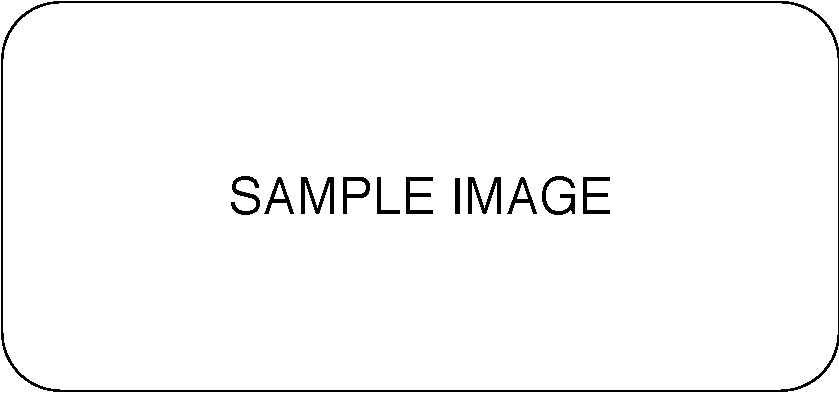
\includegraphics[scale=0.7]{Images/SampleImage.pdf}
	\caption{Structure of the test suite}
	\label{fig:syTestSuite}
\end{figure}

\subsection{Build Integration}

The next step in the development process revolved around the integration of the developed test cases in the nightly builds. The build process in Dynamics 365 for Finance and Operation is handled by a build VM that contains a build agent (that runs the computational operations of the build process), controller (that distributes the build workload to all the available agents), process template (where the build steps are defined) and definition (that specifies what you want to build, when a build should start, where the build output should be sent). The tests that a developer wants to add to the build process are specified in the build definition and are executed after the build process has proven to be successful. Test execution is organized into three activities: test setup, test execution and test end. The Trade+ project code is subjected to nightly builds that are executed every 24 hours. We decided to begin the integration process by creating a 

%********************************** %Fifth Section  **************************************
\section{Deployment}

Lorem Ipsum

%********************************** %Sixth Section  **************************************
\section{Operation (Future Work)} 

Lorem Ipsum